\chapter{Conceitos Utilizados}

\section{Tecnologia de comunicação}
A partir de todo o levantamento teórico e considerando-se o contexto do problema, a tecnologia que mostrou mais destaque, foi o Bluetooth.

Mais especificamente, a introdução do Bluetooth Low Energy (BLE) tornou tal tecnologia bem favorável ao uso para localização, devido ao seu baixo consumo energético, mantendo caracteristicas similares de comunicação.

As principais características da escolha podem ser encontradas abaixo:

\begin{itemize}

    \item \textbf{Economia e eficiência energética}

    Uma das principais vantagens da tecnologia Bluetooth para a localização indoor é sua alta eficiência energética. O custo da instalação de um sistema com BLE é baixo quando em comparação de outras tecnologias já que um dispositivo equipado com um chip de BLE pode de 1 a 2 anos com uma unica bateria moeda (\textit{coin cell}).No contexto de um armazém, a economia de custos é fundamental.

    \item \textbf{Acessibilidade e Escalabilidade}

    Como mencionado, estima-se que até 2022 400 milhões de dispositivos de localização baseados em Bluetooth sejam vendidos por ano \cite{art9}. Fazendo-o uma tecnologia prontamente acessível e com vários recursos de desenvolvimento.

    Para o contexto do projeto, uma rápida implementação é desejável. Além disso, estar presente em dispositivos atuais é um requisito, dado que se deseja a instalação do sistema com o minimo de mudança na infraestrutura atual. Bluetooth está presente na maioria dos telefones celulares, os quais poderiam se integrar ao sistema prontamente.

    \item \textbf{Precisão}

    A precisão necessária é tal que dois SKUs (Unidade de Manutenção de Estoque) em localidades diferentes possam ser diferenciados. Para isso, uma precisão de até 1m é desejada.

    Com a tecnologia Bluetooth e os algoritmos corretos tal precisão pode ser alcançada.

    \item \textbf{Latência}

    A latência no Bluetooth é elevada quando comparada à outras tecnologias. Para aplicações que precisão de localização em tempo real pode ser uma desvantagem. Entretanto no projeto em questão os ativos ficam estáticos no armazém. E a latência não se torna um problema tão grande.

\end{itemize}

\section{Propriedades do sinal}
Os principais algoritmos mencionados anteriormente exigem para sua implementação uma distância conhecida e um ângulo conhecido para um ponto de referência. No presente trabalho, será utilizado o RSSI como método principal para estimar a distância. %e o AoA para estimar o ângulo.

Quando um chip de Bluetooth recebe o sinal ele é capaz de retornar o valor da intensidade desse sinal, então a obtenção do RSSI é direta e não exige nenhum hardware adicional. Apesar de não ser o método mais preciso para estimar distância, seu custo benefício é alto.

Já para estimar o ângulo, o angle of arrival de um sinal poderia ser utilizado. Tal propriedade em conjunto com a de intensidade do sinal permite que algoritmos estimem uma localização com uma precisão maior quando em comparação a algoritmos que utilizam apenas a intensidade do sinal. Assim, apesar de necessitar de um hardware mais complexo, há um ganho significativo.

Porém, antes de entrar no nas especificidade das propriedades do sinal utilizadas, cabe um detalhamento do protocólo de Bluetooth Low Energy (BLE).
\subsection{Protocólo BLE}

O BLE funciona
% \todo{BLE protocolo}

\subsection{RSSI}
O RSSI, como uma propriedade bruta do sinal adquirida pelo stack de Bluetooth, fornece uma precisão de menos de 10m. Valor relativamente alto para a realização de localização indoor. Entretanto, é possível melhor essa precisão com algumas técnicas, em hardware, firmware e software.

Na aquisição do sinal, foi implementado uma técnica para a obtenção da intensidade do sinal em cada um dos três canais de advertising (canal 37, canal 38 e canal 39) separadamente, em contraste com a abordagem clássica de obter o RSSI de todos os canais de advertising simultaneamente, o que permite uma maior precisão no uso do RSSI. A dificuldade desse método aparece porque o padrão BLE nativo, não provém uma API para recuperar informação dos canais de advertising na recepção dos pacotes transmitidos, assim pequenos ajustes no stack de bluetooth devem ser feitos [22].

Essa técnica melhora a precisão do RSSI em relação com a obtenção de todos os sinais simultaneamente pois assim é possível fazer uma análise personalizada para cada um dos canais, mitigando efeitos de interferências entre os canais, efeitos de \textit {fading} e eventuais erros na transmissão de dados [23].

Uma vez coletada a informação dos canais separadamente, deve-se tratá-los adequadamente. Dependendo da situação, uma das formas de tratamento a seguir foi utilizadas :

\begin{itemize}

    \item Utililzar dados somente do canal que está fornecendo o maior valor de RSSI. O canal que é considerado como dando a maior precisão é o que fornece maior RSSI nesse caso:

    \begin{equation}
        RSSI_{max} = max(RSSI_{ch37}, RSSI_{ch38}, RSSI_{ch39})
    \end{equation}

    \item  Utilizar a média dos calores obtidos em todos os canais. Usando a média dos três canais, eventuais erros em um canal tem seu efeito minimizado:

    \begin{equation}
        RSSI_{average} = \frac{1}{3} \sum_{i=37}^{39}  RSSI_{ch i}
    \end{equation}


    \item Obter o valor do RSSI pela combinação de razão máxima (\textit{Maximum Ratio Combining} - MRC). Essa abordagem coloca peso nos canais de forma que a combinação resultante dê uma enfasê maior para os canais com maior leitura de RSSI do que para os canais com menor leitura, porém os com menor leitura ainda são levados em conta:

    \begin{equation}
        RSSI_{MRC} = \sum_{j=37}^{39} \frac{RSSI_{ch j} - RSSI_{min}}{\sum_{i=37}^{39}  RSSI_{ch i}} RSSI_{ch j}
    \end{equation}

    Em que o valor de \( RSSI_{min} \) foi escolhido de acordo com a mínima sensibilidade do módulo bluetooth utilizado.


\end{itemize}

A partir do valor de RSSI que foi estimado com base no RSSI dos três canais, utilizou-se a triangulação para a determinação da posição de acordo com as equações de \ref{sec:trilateracao}.

Nas imagens \ref{fig:rssi_channels_raw.png} e \ref{fig:rssi_channels_mrc.png} tiradas de [23], é possível perceber a diferença que a leitura separada dos canais pode fazer. Na imagem \ref{fig:rssi_channels_raw.png}, tem-se a leitura bruta dos valores dos canais para 500 medições, nessa caso há uma alta dispersão dos dados para um mesma distância, demonstrando a necessidade de algum tipo de tratamento dos dados.
Na imagem \ref{fig:rssi_channels_mrc.png}, utilizou-se o método do MRC descrito acima. Neste caso, há uma flutuação bem menor dos dados, o que é crítico para uma localização precisa.

\begin{figure}[H]
    \centering
    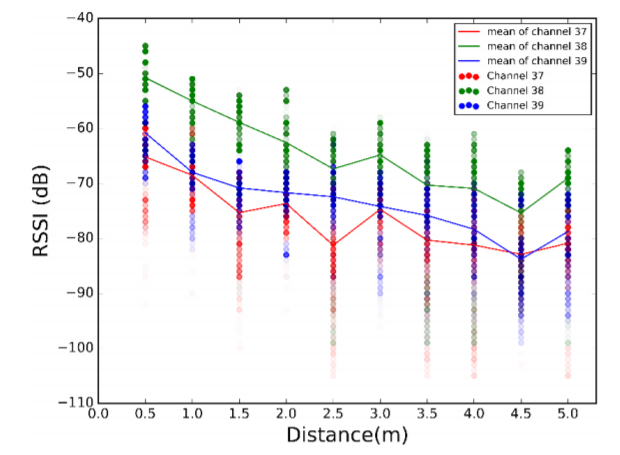
\includegraphics[scale = 1]{images/rssi_channels_raw.png}
    \caption{Gráfico de dispersão do RSSI medido para diferentes distâncias conhecidas para diferentes canais sem tratamento.  [23] }
    \label{fig:rssi_channels_raw.png}
\end{figure}

\begin{figure}[H]
    \centering
    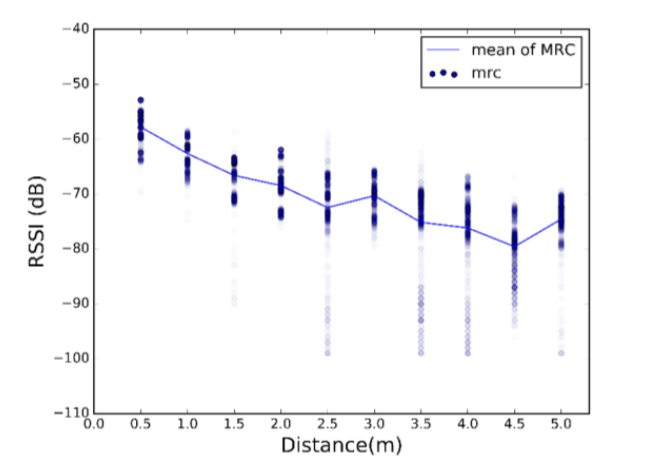
\includegraphics[scale = 1]{images/rssi_channels_mrc.png}
    \caption{Gráfico de dispersão da média do RSSI calculado por meio do algoritmo MRC [23]}
    \label{fig:rssi_channels_mrc.png}
\end{figure}



\subsection{Angle of Arrival}
Já, quanto ao Angle of Arrival, apesar de não ser diretamente utilizado na implementação da solução, dado que chegou-se em uma precisão de localização aceitável apenas com o RSSI, um detalhamento de como seria possivel obtar tal parâmetro é dada aqui.

Em primeiro lugar, para se obter a direção de um sinal é necessário um array de antenas, responsável por extrair a informação de angulo do sinal recebido. Há diversas técnicas para se obter . As mais conhecidas são: Outra que será descrita é:
% \todo{extracao AoA}
Vale ressaltar o ble 5.1
% \todo{5.1}

Nas especificações do Bluetooth anteriores à 5.1 lançada em janeiro de 2019, a obtenção do AoA exigia um hardware extra.
Entretanto, dados os recentes avanços na tecnologia agora é possivel estimar o ângulo de chegada de um sinal se o chip Bluetooth utilizado possuir suporte para Bluetooth 5.1 ou superior.

Uma alternativa para estimar o AoA para especificações anteriores à 5.1 é a utilização de um interferômetro de 6-portas, que é um dispositivo que é baseado nas superposições deslocadas de fase das ondas incidentes e refletidas em uma porta. Diferentes defasagens de fase resultam em diferentes potências nas portas de saída da arquitetura de um 6-portas \cite{art14}.

Abaixo um desenho esquemático da arquitetura de um 6-portas:

\begin{figure}[H]
	\centering
	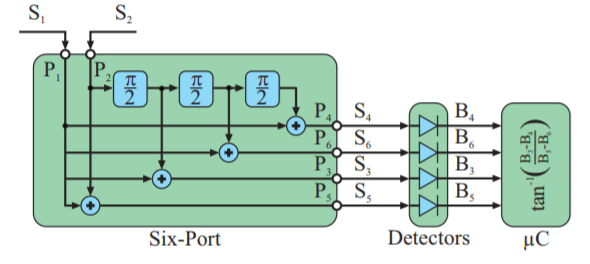
\includegraphics[scale = 1]{images/six_port_schematic.png}
	\caption{Esquemático de uma arquitetura 6-portas. Tirado de \cite{art15} }
	\label{fig:six_port_schematic}
\end{figure}

Na figura \ref{fig:six_port_schematic} os símbolos \( S_1 \) e \( S_2 \) representam os de sinais de entrada e \( S_3 \) a \( S_6 \) representam as potências medidas na saída. Já os simbolos de \( B_3 \) a \( B_6 \) representam as potências de \( S_3 \) a \( S_6 \) convertidas para tensões de base.

As equações que relacionam esses sinais são:

\begin{align*}
    S_3 & = 0.5(S_1 + jS_2) & B_3 = \left | S_3 \right | ^2\\
    S_4 & = 0.5(S_1 - jS_2) & B_4 = \left | S_4 \right | ^2\\
    S_5 & = 0.5(S_1 + S_2)  & B_5 = \left | S_5 \right | ^2\\
    S_6 & = 0.5(S_1 - S_2)  & B_6 = \left | S_6 \right | ^2
\end{align*}

A partir disso, é possível encontrar diversas propriedades úteis dos sinais incidente, tais como a a diferença de fase \( \Delta\phi\), a distância do sinal \( \Delta\delta\) e a propriedade que mais interessa para o presente trabalho, o ângulo de chegada \(\theta\) a partir das seguintes equações:

\begin{equation}
    Z = (B_5 - B_6) + j(B_3 - B_4)
\end{equation}

\begin{equation}
    \Delta \phi = \arctan \left ( \frac{B_3-B_4}{B_5-B_6} \right )
\end{equation}

\begin{equation}
    \Delta d = \lambda \frac{\arg\left ({Z}  \right ) }{4\pi }
\end{equation}

\begin{equation} \label{eq:eq_AoA}
    \theta = \sin^{-1}{(\frac{\lambda \Delta \phi}{2\pi a} )}
\end{equation}

Em que Z é um número complexo que relaciona as tensões de saída, \(\lambda\) é o comprimento de onda do sinal e \(a\) a distância entre antenas receptoras.

A referência \cite{art15} apresenta um maior detalhamento da arquitetura. Para o contexto de localização indoor, as equações forneceriam o ângulo \(\theta\) desejado.

\section{Algoritmos}

% \todo{Algoritmos}

\section{Camada de Aplicação}

% \todo{Teoria Aplicacao}
